%
% DSP Report Template
%
% (c) 2005 EMT DSP Group
%
\documentclass[12pt,a4paper]{article}
%\usepackage{dsp_report}

\usepackage{parskip}

% randausgleich bei kleinen zeichen mit wenig deckung rechts
% % http://latex.tugraz.at/latex/fortgeschrittene#optischer_randausgleich
\usepackage[activate=normal]{pdfcprot}


%
%\DSPTitle{Odometry for Wheeled Mobile Robots}
%{Michael Maier}

\usepackage{graphicx}

\usepackage{subfigure}
\usepackage{xspace}                   % space nach makro
\usepackage[left]{eurosym}            % Euro symbol
\usepackage{hyperref}

\usepackage{needspace} %preserve some space before page break, e.g. at a listings heading

\newcommand{\mbnote}[1]{\textcolor{Gray}{\textbf{\noindent M. Brandner NOTE: #1}}}
\newcommand{\mmnote}[1]{\textcolor{Gray}{\textbf{\noindent M. Maier NOTE: #1}}}
\newcommand{\MH}{\emph{``Mostly Harmless''} RoboCup Team\xspace}
\newcommand{\MSL}{Middle Size League\xspace}
\newcommand{\robocup}{\emph{RoboCup}\xspace}

\begin{document}

%% Based on a TeXnicCenter-Template by Tino Weinkauf.
%%%%%%%%%%%%%%%%%%%%%%%%%%%%%%%%%%%%%%%%%%%%%%%%%%%%%%%%%%%%%

%%%%%%%%%%%%%%%%%%%%%%%%%%%%%%%%%%%%%%%%%%%%%%%%%%%%%%%%%%%%%
%% Deckblatt
%%%%%%%%%%%%%%%%%%%%%%%%%%%%%%%%%%%%%%%%%%%%%%%%%%%%%%%%%%%%%
%%
%% ATTENTION: You need a main file to use this one here.
%%            Use the command "\input{filename}" in your
%%            main file to include this file.
%%
\begin{titlepage}

  \begin{center}
    \begin{minipage}[htb]{18cm}
      \hspace*{-2.6cm}
      
\includegraphics[width=3.3cm]{./figures/logos/LogoEMT.pdf}
      \begin{tabular}{p{10cm}}\centering{
      \Large Institute of Electrical Measurement and Measurement Signal Processing\\ Graz University of Technology
      ~\\
      ~\\}
      \end{tabular}
      
\includegraphics[width=3.3cm]{./figures/logos/TUG.pdf}
    \end{minipage}

    \Large {Bachelor's Thesis\\} %
    \vspace*{1cm} \huge{\textbf{Odometry for Wheeled Mobile Robots}\\}
    %
    \vspace*{1.0cm} 
    %\Huge{\textbf{#1}\\}\vspace*{2.5cm} \vfill
    \Large{Michael Maier\\} \vspace*{1cm}
    %
    \Large{Supervisor: Dipl.-Ing. Dr. Markus Brandner\\} \vspace*{2.5cm}%


    \begin{minipage}[htb]{18cm}
      \hspace*{-0.4cm}
      
\includegraphics[width=3cm]{./figures/logos/MH.jpg}
      \begin{tabular}{p{10cm}}\centering{
        \Large Mostly Harmless RoboCup Team \\Institute for Software Technology, \\Graz University of Technology\\
        \texttt{team@robocup.tugraz.at}\\ \texttt{http://www.robocup.tugraz.at}
        ~\\
        ~\\}
      \end{tabular}
    \end{minipage}

    \Large{Graz, \today}

  \end{center}
\end{titlepage}


\tableofcontents
\clearpage
\pagestyle{plain}


\begin{abstract}
Abstract

% 1p
\end{abstract}

\clearpage

\section{Introduction}


\subsection{RoboCup}

The RoboCup is an international research and education initiative. 
Its goal is ``By the year 2050, develop a team of fully autonomous robots that can win against the current human soccer world champion team"~\cite{robocup.org}.
It encourages research in the field of robotics, e.g.\ machine vision, machine learning and autonomous systems.

%|| to Apollo Program.

Every year a world championship is accomplished by a conference in a different city around the globe.
In addition, various local competitions and conferences are held by local groups.

The RoboCup is divided into three parts: RoboCup Soccer, Rescue and @Home.
Every division is divided into several leagues targeted at different challenges.

%1/2 page

\subsection{\MSL}

In RoboCup Soccer the \MSL is most challenging.
The robots have to be fully autonomous.
All sensors, actuators and computation are on board and no external input is allowed.
A Team consists of maximal 6~robots with a size of max. $50\times50\times80$\,cm$^3$.

The game is played on a field of $12\times18$\,m$^2$ and lasts $2\times15$~minutes.
The game field surface is usually carpet.
The \MSL is the only league where an official FIFA ball is used.
Objects are distinguished by colour, the game field is green with white lines, robots and referees are black and the ball is red.

The rules are the official FIFA rules~\cite{msl-rules} with slight adaptations for robotic players.
The rules are tightened every year to keep up with the technological progress. 
For instance the field size has grown from $6\times8$\,m$^2$ to $12\times18$\,m$^2$ since the introduction of the \MSL.

More than 20 teams from all over the world participate in the \MSL, almost all with academical background.

% 1/2 p

\subsection{\MH}

The \MH participates in the \MSL. 
Its name is a reference to the ``Hitchhiker's Guide to the Galaxy'' by Douglas Adams~\cite{h2g2}.
It was founded at Graz University of Technology at the Institute for Software Technology in 2003. 
This RoboCup team consists solely of students and acts as a platform for master's, bachelor's thesis and seminar projects.
Currently more than 30~students are working on the robots in their free time.

It regularly participates at European championships as well as World Championships.
At RoboCup~2009, which took place in Graz, the team advanced a round in the World Championship for the first time.
The third place in the technical challenge was won too.



% 1/4 p

\subsection{Current robot platform: Krikkit}

The ``Krikkit'' robot platform was built in 2006.%~\cite{}. 
It was designed solely for playing soccer, in contrast to the old, multi-purpose research robot platform.
Nearly all components from electronics to mechanical parts are developed in-house.
Four robots were built and made their d\'ebut at the World Championship 2006 in Bremen.

Some of the main features of the ``Krikkit'' robot are shown in \autoref{fig:krikkit}.

\begin{figure}[ht]
\begin{center}
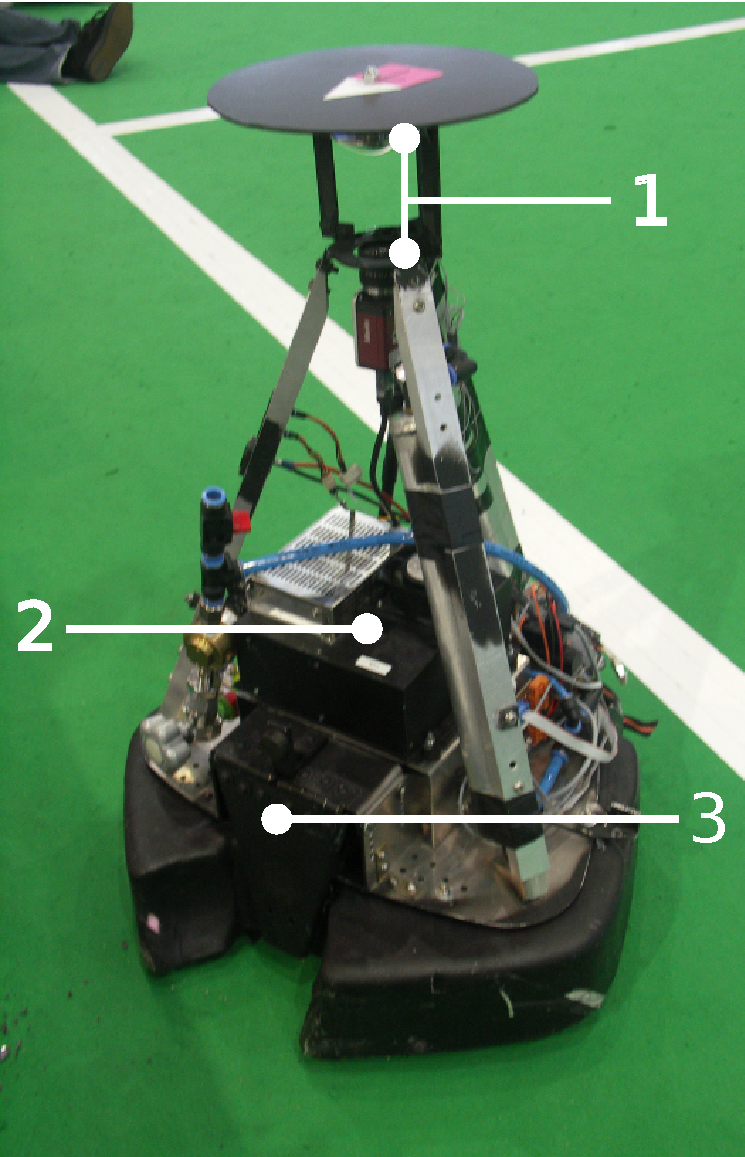
\includegraphics[width=0.5\columnwidth]{figures/krikkit.pdf}
\caption{\label{fig:krikkit}
Krikkit robot. Omni-vision with camera and mirror~(1); Industrial PC~(2); Pneumatic kicker~(3); Omni-drive is below the black bumper.
}
\end{center}
\end{figure}

It has a $360^\circ$ omnidirectional vision system via a firewire-camera pointing upwards to a hyperbolic mirror.\\
Its brain is a standard mini-ITX industrial PC.\\
A powerful pneumatic kicker, with a~200\,bar pressurised air bottle as supply, enables the robot to kick the ball approx. 10\,m forward.
The kicks were such powerful that the vibrations destroyed the former--used hard disks now replaced by SSD~storage.
Additionally, every kick caused a camera blackout of nearly 2~seconds due to the vibrations.\\
Its drive system is also omnidirectional and is based on self-designed Mecanum wheels~\cite{mecanum2007}. 
The $45^\circ$\mbox{-}Arrangement of the wheels (see~\autoref{fig:mec-wheel}) promised smooth and vibration-free operation.
The three wheels are arranged in $120^\circ$\mbox{-}steps (see~\autoref{fig:omnidrive}) and are driven by a 200\,W brushless~DC motor for each axis.
Due to the nature of omni-wheels, the robots are able to move in any direction and any orientation.\\
The motors and all other electric components are supplied by a smart battery system~\cite{krammer06} with NiMH rechargeable batteries.
All electronic components are connected via CAN-bus.

\begin{figure}[hb]
  \begin{minipage}{0.45\textwidth}
   \centering
    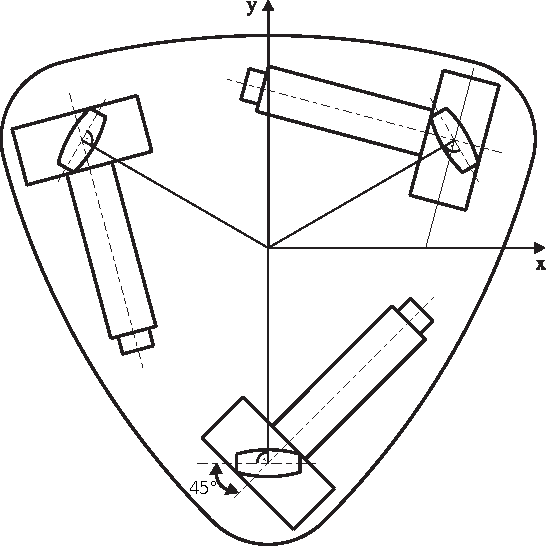
\includegraphics[width=1\textwidth]{figures/krikkit_drive_angles}
    \caption{\label{fig:omnidrive}Omni-drive schema of the Krikkit robot. The Mecanum wheels have their $45^\circ$~small wheels arranged in $120^\circ${-}steps around the centre.
    \cite{mecanum2007}}
  \end{minipage}\hfill
  \begin{minipage}{0.45\textwidth}
   \centering
    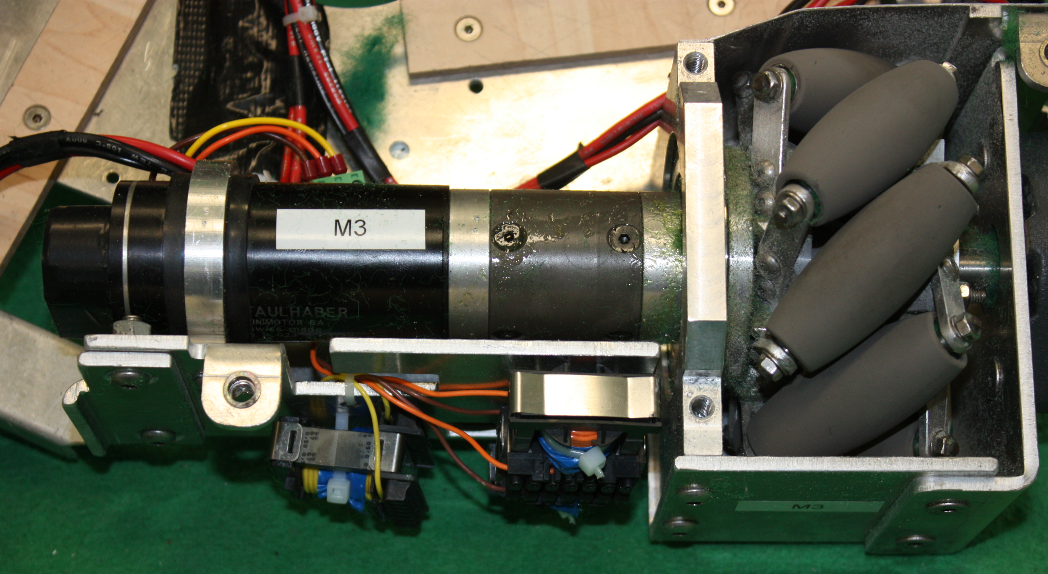
\includegraphics[width=1\textwidth]{figures/Omniwheel_drive.png}
    \caption{\label{fig:mec-wheel}Photo of one of the three Krikkit power trains, visible are from left to right: Motor, gearbox and Mecanum wheel.}
  \end{minipage}
\end{figure}


The Krikkit robots served well for four years and much was learned.
Before RoboCup~2009 in Graz a major mechanics overhaul was done.
In the meantime all major electronic components reached the end of their life cycle also.
With the knowledge gained, lost and acquired again the successor of the Krikkit generation is in development now.
    

\subsection{In development: Krikkit3G}

The next generation of robots is in development since mid-2010.
It will be a direct successor of the Krikkit generation, therefore the name \emph{Krikkit3G}.

\Needspace*{4\baselineskip}
The successful concepts are adopted nearly unchanged:\nopagebreak[4] %% FIXXME only works inside sentences, want not to break up before the listing
\begin{itemize}
  \item omnidirectional drive with the three Mecanum Wheels
  \item the omni-vision system
  \item pneumatic kicking concept
  \item the use of a standard mini-ITX industrial PC
  \item modularity of all components
\end{itemize}

The new robot design focuses on the strict modularity of all components.
It has been shown that fast disassembling and replacing of critical components is crucial in the fast-paced tournament environment.
The power train has especially been modularised, the wheel, gearing, motor and motor electronics can be swapped as a whole group.

Tests showed that the smoothness of the Mecanum wheels had been insufficient due to manufacturing imprecision.
The resulting vibrations should be filtered out by an independent wheel suspension.

%  bumpers ?

For the kicking system the pneumatic principle was kept, but it is now much more versatile. 
It can switch between high and flat kicks at full power and side-kicks are also possible now.
Featuring a new ball guidance system allows grabbing the ball for a short moment.
This feature becomes especially useful when decelerating with the ball.
The vibrations from the kicker, disturbing the camera, should also be reduced by an active final position dampening system.
Nevertheless short disturbances in the vision system, due to the vibrations, will remain during the kicks.

Big changes have been made in the electronic sector.
A new microcontroller core (An ARM Cortex~M3) is used on every component, which replaces the different microcontroller architectures used before.
The smart battery system also got a major upgrade, featuring even smarter batteries.

In the mechanical design space is now also provided for an improved odometry system, which will be developed based on this work.

% FIXXME get newer rendering, where camera holding bars are correct.
\begin{figure}[b]
\begin{center}  
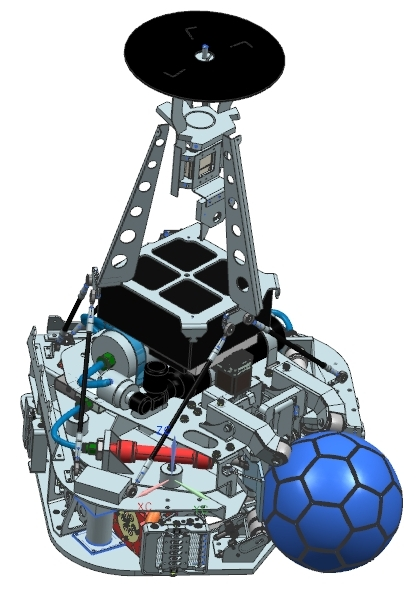
\includegraphics[width=0.5\columnwidth]{figures/Krikkit3G.jpg}
\caption{\label{fig:krikkit3g}
Rendering of the currently in construction Krikkit3G robot (Without outer hull).
}   
\end{center}
\end{figure}


% 1p

\subsection{Odometry}

%  Definition
%  Verwendungsmoeglichkeit
%    Lokalisierung
%      higher framerate than cam
%      backup-system for cam
%    Motion control
%      anti-slip regulation

Odometry, better known as path measurement is important for every moving vehicle, especially robots, which need to know where they currently are. 
The best known odometry measuring is used in cars as kilometre reading on the tachometer.

For autonomous mobile robots odometry plays an even more important role.
Together with the vision system and the compass it is a part in the sensor fusion for building the world model.
In the current Krikkit software, it fulfils the following purposes:
At first it acts as an initialisation vector for the vision system when comparing two camera frames for calculating the offset between them.
The second important role comes from the high frequency of odometry data.
Odometry data is provided with a frequency of 50\,Hz. 
This is much faster than the currently used vision system (15~-~25\,Hz). 
Therefore its values are added to the last known position in the world model for the time between two camera frames.
At last it acts as a backup system for the mainly vision based localisation system in case of camera blackouts e.g.\ blurred images due to the vibrations from a kick or a collision.

There are more possible use cases for odometry not implemented yet e.g.\ anti-slip regulation for every single wheel.



\subsection{Motivation for this work}
\label{motivation}
  
Current odometry systems of the Krikkit generation are based on the rotational speed of the wheels.
This has the major disadvantage of the accuracy being bound to the slip of the wheels. %FIXXME English being okay?
The problem is the non-uniform structure of the game field carpet, which has different slip factors in each direction.
Due to the different speeds and angles of the Mecanum wheels it leads to deviations even when driving a straight line.
The errors accumulate over time, resulting in $90^\circ$~deviation on 10\,m straight distance driven.

\Needspace*{4\baselineskip}
Therefore an wheel-independent odometry system has to be developed.
The goals of this work were:
\begin{itemize}
  \item Gathering requirements for a sensor
  \item Search for different types of sensors
  \item Implementation and validation of a prototype
\end{itemize}


\subsection{Requirements for a new type of odometry sensor on the Krikkit/3G platform}

The \MSL provides an ideal testbed for mobile robotics.
The main demands in robotics are miniaturisation, low cost, energy usage and robustness against the environment.

\Needspace*{4\baselineskip}
The range of application in the \MSL demands the following design parameters for an odometry sensor: %% FIXXME no page break here!
\begin{itemize}
  \item must deliver linear and rotational accurate data in three degrees of freedom
  \item must work on green carpet, other surfaces are bonus
  \item must not emit radiation or other disturbing effects irritating other robots or humans
  \item resistance against dust from the carpet abrasion
  \item shock resistant
\end{itemize}

The carpet is a particularly hairy concern, as its choice is up to the event organizer.
The only restriction in the \MSL rules and regulations~\cite{msl-rules} is: green.
Therefore the game field surfaces differ in colour and surface roughness on every event.
Colours from bright green over dark teal to nearly grey have been seen over the past years.
The roughness is another chapter.
It ranged from a very even felt with a roughness of maximum~2\,mm to an artificial grass like carpet with 15\,mm long hairs. 
Depending on the carpet the robot sinks in some millimetres, which also affects the clearance height.

The \MH requirements for a new odometry sensor are speeds of at least 5\,m/s at an operating frequency of at least 50\,Hz.
From the software side it would be highly appreciated if the sensor delivered data quality information.
Data quality information is crucial for the sensor fusion to recognize and de-prioritize erroneous data.
The \MH had bad memories about a malfunctioning compass ruining the world model.
At last the \MH has very tight budgetary limitations depending on external sponsors and due to being a student team.
The sensors have to be cheap enough to be affordable for series for up to six robots.


On the Krikkit3G robots the available space is limited to $50\times50\times110$\,mm$^3$ for each of the three proposed sensor mount points.
The Krikkit3G robot, similar to the old Krikkit generation, has a clearance height of 20\,mm.
Due to the new independent wheel suspension the operating range of the sensor must be greater than $\pm 5$\,mm of the reference plane.
Data must be output on the robot's CAN-bus.
As power supply only two DC lines with 24\,V and 7\,V are available at reasonable currents.





\clearpage
\section{State of the art in odometry measurement}

When determining the position or movement of a vehicle, there are the following options: 
Relying on global or relative position measurement.

The best known global position measurement is the Global Positioning System GPS.
This is widely used for robotics in outdoor applications where a GPS signal is available.
Indoors other known landmarks can be used.
In RoboCup the well-known shape of the soccer field is used for global reference.
Without exception every soccer robot uses the features of the game field e.g.\ the goals, lines and corner posts for orientation.\\
Other global approaches for gathering position data are compasses and gyroscopes.
They also deliver global data, but orientation and not position. 
This approach delivers only one of the three needed degrees of freedom, but it can complete the missing dimension.

% - global positioning
%   GPS
%   Compass
%   gyroscopes
%   relative position to known landmarks
%   - poles from 2006
%   - lines on the game field

For relative position measurement there is the choice to measure distance, velocity or acceleration.
Every approach has its advantages depending on the use case.
When aiming for the travelled distance it is not wise to measure acceleration, hence the measurement errors would sum up quickly due to the twice integration.\\
When measuring acceleration there is the choice between industrial grade accelerometers as used e.g.\ in aeroplanes and consumer grade accelerometers based on the piezoelectric effect.\\
Speedometers exist in various implementations based on the Doppler effect e.g.\ radar.\\
Distance metres can be mechanical or optical.
The simplest mechanical distance metre is a measuring tape, or when used on moving vessel, the log-line of a sailing ship used for speed measurement.
In the last decade another electronic approach was developed: optical distance metres based on comparing images for translational displacement, as used in optical computer mice.

% - relative positioning
%   - acceleration
%   - velocity
%   - distance
%   accelerometers
%   speedometers relying on the Doppler-effect
%   mechanical distance meters (like in cars or early computer mice)
%   optical distance meters based on comparing images for translational displacement, as used in optical computer mice


\Needspace*{4\baselineskip}
Every approach has properties to evaluate:
\begin{itemize}
  \item maximum and minimum speed capability
  \item maximum and minimum acceleration
  \item number of dimensions of movement data one sensor delivers
  \item linearity and deviation of data
  \item length of time of a single measurement
  \item time lag between measurement and data availability
  \item highest possible frequency of measurements
  \item resilience against reference surface distance changes
  \item maximum and minimum distance to reference surface
  \item surface state requirements
  \item resilience against environmental changes
  \item influence of the sensor on the environment 
  \item size and power requirements of the sensor
  \item cost of the sensors for three dimensions
\end{itemize}

In preparation for this work a lot of sensor types, both industrial and consumer grade, were evaluated for the use in the \MSL based on these properties.


\subsection{Possible new odometry sensors types}

In this section technologies to be considered as improved odometry sensor are described in general.
The reasons for selecting a particular sensor type for evaluation in this work are explained in~\autoref{decision}.


\subsubsection{Accelerometers}

Accelerometers consists mainly of flexible mounted masses, which are under the influence of a force.
If the mounting consists of springs, the displacement is linear to an applied force.
This displacement is then measured.
Under normal circumstances on earth every object is under the influence of the gravitational force.
Therefore~1\,g must be subtracted from the result.

In commercial sensors piezoelectric elements are used to convert the force into a signal.
In the last years the use of micro electro-mechanical systems (MEMS) has been increased significantly.
Sensors for three dimensions are now available in tiny package formats at low cost for consumer applications.

\subsubsection{Gyroscopes}

Gyroscopes are inertial sensors, which detect the change of position.
Historically they consisted in a flywheel mounted in a Cardan suspension.
Once spinned up they remain at their orientation, based on the principles of conservation of angular momentum.

Today they are implemented as MEMS similar to  the before mentioned accelerometers.
Often they are even combined with accelerometers in a single chip package to 6-dimensional sensors.


\subsubsection{Ultrasonic Doppler velocimeters}

Ultrasonic Doppler velocimeters work similar as ultrasonic distance sensors.
Ultrasonic distance sensors were used in the first robot generation of the \MH for collision detection.

As on every Doppler measurement, its accuracy is directly dependent on the used wavelengths.
At ultrasonic sensors wavelengths around~100\,kHz are used. 
This leads to significantly more accuracy as e.g.\ Microwave Doppler sensors~\cite{ultrasonic}.

When working with ultrasonic sensors on mobile systems, one thing has to be taken into consideration: 
As on every wave-based system, the relative speed of the medium~(air) has to be considerably smaller than the wave speed ($v \ll c$).
Through the relatively low velocity of sound, only speeds up to~30\,km/h are feasible because of the head wind and turbulences~\cite{ultrasonic}.

Also, ultrasonic Doppler velocimeters subtle to vibrations due to low frequencies~\cite{agri}.

The main use today is in liquid flow measurements.



\subsubsection{Microwave Doppler velocimeters (Radar)}

Radar is an umbrella term for object detection systems utilizing electromagnetic waves from 300\,MHz up to 3\,THz~\cite{nrt}.
It can be used to measure the distance of objects and also their speed through the Doppler effect.
Depending on the object distance, different wavelength are used.
For short-range measurements short-range microwave sensors with~24\,GHz are used e.g.\ radar guns and also for speed measurements on moving vehicles itself~\cite{s_r_radar}.

\subsubsection{Laser interferometers}

Speed measurement with laser interferometry is divided into two approaches.
One called Laser Doppler velocimetry and the other is referred as Laser Doppler vibrometry.

In Laser Doppler velocimetry two coherent laser sources are intersected on the moving target surface at different angles.
The interference of the two beams creates a set of straight fringes. 
Particles of the surface, moving through the fringes, reflect light on the constructive interferences.
The resulting frequency is then captured by a photo diode~\cite{laser_vel}.

% source: WP

In a Laser Doppler vibrometer the beam is split into two coherent beams.
One beam is reflected and then interfered with the second beam and afterwards collected in a photo diode. 
The frequency shift between the two beams results in an overtone at the detector.

% source: WP

%\subsubsection{One-dimensional Optical Spatial Frequency Filtration}
%1/4



\subsubsection{Industrial/Custom-build optical speed sensors}

The operation of an optical speed sensor is based on comparison of sequentially acquired images from a surface.
From the images, features are extracted, and their position is compared with similar features on the next frame. 

Such optical systems are common in industrial and consumer sensors.
Examplary uses are speed sensors for conveyor belts.

The components of an optical speed sensor are usually a high-speed camera, acquiring the images from the surface, and a Digital Signal Processor (DSP) for analysing the images.
In industrial systems the cameras are usually fixedly mounted and are connected to an external processing device~\cite{opt_vel}.

When the surface contrast is not sufficient to extract enough features for tracking, a little trick helps.
Every sufficiently rough surface creates a so-called \emph{speckle} when illuminated with a coherent light source.
This comes from the interference of reflected light waves with different phases due to the roughness of the surface.
Therefore illumination with a laser light source increases the contrast a lot on otherwise low contrast surfaces.
This is used e.g.\ in laser speckle strain measurement~\cite{strain}.

When developing such a system from scratch, a lot of time and effort is needed.
This has been shown by the development of an optical slip-angle sensor~\cite{Hrach2006} for the TUG~Racing~Team.

% 1/4
\subsubsection{Optical mice}

The most common optical speed sensor is used in newer computer mice.
Historically computer mice featured a rolling ball with two attached axles (one for each axis), whose rotations are turned into coordinates.
In the last 10~years this mechanical principle has been superseded by a strictly electronic approach.

A standard optical mouse consists in a tiny camera taking images of the surface illuminated by an LED.
The processing of the images is done by an integrated DSP.
The sensor outputs movement data to an external microcontroller, which also handles the mouse buttons and translates all data to the~USB or PS/2 protocol.

At the time of the search~(2008), the fastest gaming mice had a maximum speed of 1.1\,m/s.\\
They operate at speeds up to 7\,000\,Hz.
Another advantage is their small size and minimal power requirement.\\
Being constructed as an exact gaming device also has disadvantages for RoboCup use:
To allow relocating the mouse very fast while lifting off, the best mice used for gaming are designed with a very short working range of only 2\,mm.

Laser mice use the same principle as the before mentioned laser speckle sensor.
The only difference to normal mice is the use of a coherent laser source as illumination instead of an LED.
The sensor itself remains the same, but due to the higher contrast achieved through the speckle, they work on more surfaces than common optical mice.

 
% 1/2

\subsection{Current implementations used in RoboCup}

\subsubsection{\MH}

The current odometry system of the Krikkit robots is based on rotary encoders attached to each of the axles. 
The rotary encoders are needed for motion control, and odometry data fells off as a by-product.
The data from all three rotary encoders is collected by the motion controller, converted into $dr$,~$ds$,~$d\phi$ - coordinate values and send out on the CAN-bus.

Relying on the mechanical contact between the ground and the wheels brings various problems, as already mentioned in~\autoref{motivation}.
An effect known from all wheels is the slip on accelerating and braking.
The use of Mecanum wheels complicates the relationship between robot and the floor.
Due to different speeds of every wheel even when driving a straight line, resulting from the $120^\circ$\mbox{-}steps the wheels are mounted, every wheel has a different amount of slip.
Another factor not to be underestimated is the distinctive direction of the fibre of the carpets~\cite{mecanum2007}.
The direction of the fibre results in globally different friction factors in every direction.

Another common construction error of the power train used in the Krikkit robots was a loose connection between the gearing box and the motor.
The rotary encoders are mounted on the motors and not on the wheels.
When the connection between motor and the wheel got loose, the rotary encoders delivered only the rotation of the motor and not the distance covered by the wheels. 
This resulted in complete disorientation of the localisation software during an overrunning motor.\\
But faulty mechanics are not always responsible for this type of error, it is sufficient when a wheel looses contact with the ground for a moment.
This can happen when running aground on a lost screw or other parts lying around the game field or when two robots become wedged together.

For global positioning, in addition to the vision system, a compass is used.
Most of the time this works well, but once in a while we had problems with massive steel girders below the game field.
Due to the over-weighting of compass data, the localisation software went amok.
Therefore data quality information would be highly appreciated from every sensor used.

\subsubsection{Other teams}

Rotary encoders on wheels are widely used, e.g.\ in the team ISocRob~\cite{isocrob}.
Other teams like IsePorto~\cite{iseporto} also accomplish the rotary encoders with a compass.

To counter at least the problem with the overrunning wheels when accelerating, e.g.\ the Iranian Team ADRO~\cite{adro} uses a second set of wheels for measuring odometry data.

The use of consumer computer mice in the \MSL has been tested by the Milan~Robocup~Team.
They used two optical mice mounted on the bottom of the robot.
The main advantages of this approach are the independence of the wheels and the low cost.
The availability of more dimensions than needed allowed for the corrections of non-systematic errors~\cite{two_mice}.

Accelerometers are used in other leagues, e.g.\ the RoboCup Rescue League or in the Standard Platform League with humanoid robots.
They are used only for inertial informations, not yet for navigation~\cite{zadeat}.


\subsection{Decision for a type of sensor}
\label{decision}

The focus lied on cheap consumer-grade sensor based solutions, due to the hefty price for industrial sensors.
Advantages of industrial solutions would be their robustness and in most cases their native CAN-bus interface.
But the big disadvantages of industrial sensors are the their size, weight and power requirements.
Finished industrial radars, laser interferometers and optical speeds sensors mostly use 230\,V~AC, require an external processing unit and are simply too big and heavy for middle size robots~\cite{laser_vel, opt_vel, s_r_radar}.

The approach of developing an optical sensor from scratch was shown to be successful for the automotive environment~\cite{Hrach2006}.
But it would need a lot of time and effort to shrink the gadget enough to fit inside a middle size robot.
At last, the components involving the camera and the needed FPGA-processor would be unaffordable for even one robot.

On ultrasonic sensors, most commercial sensors have $> $30\,cm surface distance, we have 20\,mm.
Reflections are another problem in ultrasonic measurement, we must use at least~3 sensors in close proximity to each other.
And due to the expected air turbulences close to the wheels as well as the reflection problem, the ultrasonic approach was rejected.

The main criterions against radar sensors are the very different reflection rates on different undergrounds (carpet, wood, concrete, steel, \dots).
The underground below the carpet is not known prior to a tournament, therefore the sensor is not guaranteed to work.
Other disadvantages are low accuracy at low speeds, and that radar is disturbed by nearby moving objects.

At time of search, consumer grade accelerometers/gyroscopes were not accurate enough to counter the summation errors.
An industrial Xsens~\cite{xsens} sensor would have better accuracy, but with a price tag of~\euro\,1.000 it was out of our budget.


The use of custom-build laser interferometers, especially vibrometers was considered.
The Institute of Electrical Measurement and Measurement Signal Processing does some work in this field.
The approach looked promising, but was not followed due to lack of time.

Mouse sensors were considered promising from the start of this project.
They are cheap, and fit into the size and power requirements of a middle size robot.
The disadvantages of missing range and maximum speed could be negated by replacing their optics.
By adding more magnification and setting the focus plane farther away from the sensor, maximum speed and range could be extended.\\
With the use of two sensors, the needed three degrees of freedom can be reached with extra redundancy. 
The \MH requires odometry data delivered on the CAN-bus, not the mice's native USB.
To convert four dimensions of data from two sensors into the needed $dr$,~$ds$,~$d\phi$ - values on the CAN-bus, a microcontroller controlling the two mice sensors is mandatory.\\
The needed microcontroller-programming and skills in electrical measurement fit the telematics area ideally, so the approach with consumer mice with replaced optics was chosen.
And last, but not least we got a sample mouse sensor sponsored from a friendly German RoboCup team, where an exhaustive data sheet was available~\cite{adns}.



%  entscheidung fuer einen Sensortyp
%    - why/why not...
%    - ...
%    - ...
%        2G spitzenvibration -> no

\clearpage
\section{Sensor design}

The task was the following: Develop an odometry sensor from a given mouse sensor.
At the beginning of this project, we got a prototype sensor sponsored from (\$ German RC team FIXME).

It consisted of a mechanically modified Razor~Copperhead laser~mouse.
In this mouse type, a sensor from Avago~Technologies is used, the ADNS-6010.
The sensor and illumination were dismounted from its~PCB and relocated in a new casing because of mechanical size constraints (see \autoref{fig:m-casing}.
It was reconnected to its PCB via thin enamelled copper wires.
It still worked, although the recommended distance to some circuit elements was exceeded considerably due to the 'extension' of the pins.

\begin{figure}[hb]
\begin{center}  
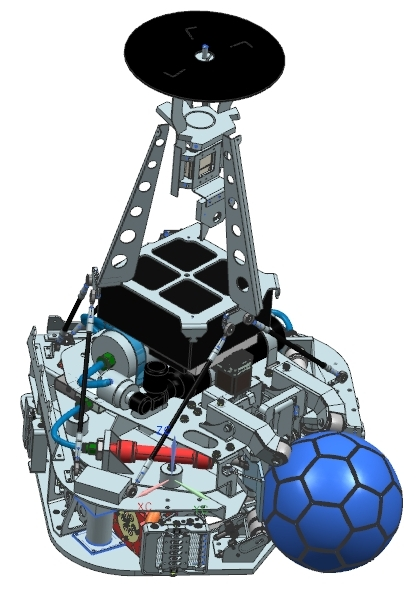
\includegraphics[width=0.5\columnwidth]{figures/Krikkit3G.jpg}
\caption{\label{fig:m-casing}
Prototype sensor from (\$ German RC team FIXME).
The Sensor~IC and the illumination was relocated from the PCB~(1) to an extension mount~(2).
}   
\end{center}
\end{figure}

Two modifications were to make: Providing a CAN interface instead of USB, and creating a new optics system.
For the new optics system, access to raw sensor image data is needed for focussing the system.
Reading out raw image data is not possible via the mouse's USB interface, only directly via the SPI~(Serial Port Interface) of the sensor chip.
Therefore it was chosen to remove the sensor chip from the mouse, and connect it directly to an external microcontroller.
This kills two birds with one stone.
The microcontroller can provide a CAN-bus interface, and provides direct access to the sensor.



We used an Infineon XC164-CM microcontroller evaluation board~\cite{xc}, of which several were available in the \MH.
For development, the microcontroller board is connected via its serial port (RS-232) to a host computer.
For the mouse sensor, a custom PCB with minimal needed circuit and the needed connections to the microcontroller was designed.
The electronics part of this work is described in~\autoref{electronics}.

The optical changes to the system with design and implementation are described in~\autoref{optics}.



The 
  - implementing the communications protocol from XC to ADNS in the microcontroller software
  - create a PCB for ADNS with minimal needed circuit.
  - calculate the needed optical system
  - 


block diagram
  ADNS + optic
  XC
  PC


\subsection{Electrical design}
\label{electronics}

Short text describing electrical layout


\subsubsection{ADNS 6010 laser mouse sensor}

specs

workflow diagram (from data sheet)

ADNS-testplatine
  requirements

  circuit diagram

  PCB drawing

\subsubsection{XC164CM microcontroller}

Specs etc

XC-164 eval board 
  Image from datasheet

Wiring of the Evaluation Board

  block diagram

  circuit

The CAN interface of the microcontroller is only needed on the final implementation on the robot, therefore it is not connected at the moment.

\subsection{Optical system}
\label{optics}
  requirements

micro-bench system

Sketch

\subsubsection{Optical path calculations: Original mouse setup}
\subsubsection{Optical path calculations: 2-Lens setup}
\subsubsection{Optical path calculations: Telecentric setup}
\subsubsection{Sensor mounting and calibration}

Sketch with adjusting screws in all dimensions

calibration process
  laser

\subsubsection{Lens 2 and aperture mounting}

manufacturing drawing

\subsubsection{Illumination}

  Why here?
  types of LEDs and Lasers used
 
  Illumination PCB

  circuit

  PCB print

\subsection{Software}

\subsubsection{Microcontroller-software}

  XC-Code
    requirements
    firmware catch

    image streaming

    motion data streaming
      + reference sensor

\subsubsection{PyQT GUI}

\subsubsection{Octave analysis scripts}

\section{Experimental setup}

- requirements

\subsection{Mechanical design of the testbed}

block diagram

\subsection{Motor and disk}

\subsection{Reference speed sensor}
      Picture of sensor from Datasheet
      electrical setup used

\subsection{Microcontroller and host PC}      

\clearpage
\section{Experimental results}

\subsection{Illumination tests}

\begin{itemize}
  \item Laser
  \item Studio Spotlight
  \item ultra-bright white LEDs
  \item IR-LEDs
\end{itemize}

\subsection{Non-telecentric tests}

\subsection{Telecentric tests}

\subsubsection{Carpet 1}

\subsubsection{Carpet 2}

\subsubsection{Carpet 3}

\subsubsection{Game field lines}

\subsection{Interpretation}

  plots
  ergebnisse

\clearpage
\section{Conclusions and outlook}

  evaluation of a combination of IR-LED illumination and Laser illumination

  newer sensor ADNS-90xx

  mechanical limitations
    size constraints
    dirt cleaning...
  electrical requirements
    new architecture: ARM
    also include illumination control in uC
      use of the shuttered illumination for higher power 
      use of both LEDs and Lasers for white lines
  software algorithms: compute 3 dimension out of 2/4/6

ca 3-5p


summe gesamt 49 Seiten (ohne abstract, inhaltsv, bibl.)


%--------------------------------------------------------%
% Bibliography
%--------------------------------------------------------%
\clearpage
\addcontentsline{toc}{section}{Bibliography}
\label{Bibliography}
\bibliographystyle{plain}
\bibliography{literature}
%
\end{document}

% vim: spell spelllang=en_gb:
